\documentclass[journal]{IEEEtran}
\usepackage[T1]{fontenc}
\usepackage{mathptmx}
\usepackage{amsmath,amssymb,graphicx,booktabs,cite,float,url}
\setlength{\textfloatsep}{10pt plus 2pt minus 2pt}
\setlength{\dbltextfloatsep}{10pt plus 2pt minus 2pt}
\setlength{\intextsep}{8pt plus 2pt minus 2pt}
\raggedbottom
\hyphenation{multi-modal land-slide back-scatter}
% ---------------------------------------------------------------------------
% DRAFT 2026-11-12. New method and dataset (DLR S1/S2 benchmark). The earlier
% Haiti dual-orbit manuscript is kept unchanged in main.tex.
% All numbers are single-run test scores (seed 42, checkpoint chosen by
% validation IoU, one test per model) from
% experiments/dlr_official6_faithful_20261110/results*/<arm>/test_metrics.json.
% Our-method numbers are macros; they currently hold arm EPRM_W and must be
% updated if the final configuration changes.
% ---------------------------------------------------------------------------
\newcommand{\oursAP}{77.58}
\newcommand{\oursIoU}{56.10}
\newcommand{\oursFone}{71.88}
\newcommand{\oursInd}{70.84}
\newcommand{\oursSpt}{48.47}
\newcommand{\oursP}{74.8}
\newcommand{\oursR}{69.2}

\begin{document}
\title{Cross-Event Optical Relation Distillation for SAR Landslide Mapping}
\author{Anonymous Authors}
\maketitle

\begin{abstract}
Optical imagery maps landslides most accurately, but clouds often leave synthetic aperture radar (SAR) as the only rapid observation after a disaster. We use optical data only during training to improve a SAR landslide mapper that receives SAR backscatter and terrain at inference. Landslide inventories are collected event by event, and a SAR network trained on them learns to recognize the training events rather than landslides. Conventional distillation from an optical teacher does not resolve this: the teacher reproduces the training labels, and most optical content is not observable in SAR. We find that students improve when they do not copy the teacher's pairwise region relations. We therefore distill only the distribution of each region's similarities to regions of other disaster events, measured by a closed-form one-dimensional Wasserstein distance, and add event-shared prototypes to the student decoder. On the official split of a 23-event Sentinel-1/2 benchmark, the student reaches \oursIoU\% intersection over union (IoU) and \oursAP\% average precision (AP) with SAR and terrain input only, compared with 52.20\% and 72.91\% for the same U-Net trained without optical data.
\end{abstract}

\begin{IEEEkeywords}
Knowledge distillation, landslide mapping, privileged information, synthetic aperture radar (SAR), Sentinel-2.
\end{IEEEkeywords}

\section{Introduction}
SAR supports landslide mapping when clouds or darkness prevent optical acquisitions during emergency response~\cite{Mondini2021,Handwerger2022,Amatya2023}. Convolutional networks map landslides from SAR backscatter~\cite{Nava2022DL,Nava2022Attention}, yet a recent multi-sensor benchmark shows that optical features remain clearly more accurate than SAR features, and that SAR models degrade most on events not represented in training~\cite{Orynbaikyzy2025}.

Training archives frequently contain co-registered optical imagery even when an emergency map must rely on SAR. Learning with privileged information and knowledge distillation (KD) exploit such training-only inputs~\cite{LopezPaz2016,Hinton2015}. Remote-sensing KD transfers predictions, features, or attention between modalities~\cite{Kieu2026DIS2,Sun2027,Lan2025ACAM,Zagoruyko2017}, and relational KD transfers similarities between samples~\cite{Park2019RKD,Tung2019SP,Aslam2024PKDOT}.

Two properties of landslide data limit these approaches. First, inventories are grouped by triggering event; a SAR U-Net reaches 90.9\% IoU on validation patches from its training events but 52.2\% on test events. Second, a multimodal teacher fits the training labels almost exactly, so its outputs carry little information beyond the labels, while its features encode optical evidence that SAR cannot reproduce. We observe that students which reproduce the teacher's pairwise region relations more closely generalize worse to new events.

We therefore transfer relational structure rather than content, and only its distribution across events. Our contributions are:
1) a cross-event relation distillation that matches, for each region, the distribution of its similarities to regions of other events with a closed-form Wasserstein distance and no pair correspondence;
2) event-shared prototypes in the student decoder that give this relational structure a deployable, event-independent form;
3) an analysis on a 23-event benchmark showing why output, feature, and pairwise relation transfer underperform for event-grouped landslide data.

\section{Method}
\subsection{Problem Formulation}
Let $X_s$ denote the student input: pre- and post-event Sentinel-1 VV/VH backscatter, elevation, and slope (six channels). The teacher additionally receives pre- and post-event Sentinel-2 bands $X_o$ (twelve channels). Both networks follow the U-Net of~\cite{Orynbaikyzy2025,Ronneberger2015}. The teacher is trained with the segmentation loss and then frozen; the student is deployed on $X_s$ only. Fig.~\ref{fig:method} summarizes the method.

\begin{figure*}[!t]
\centering
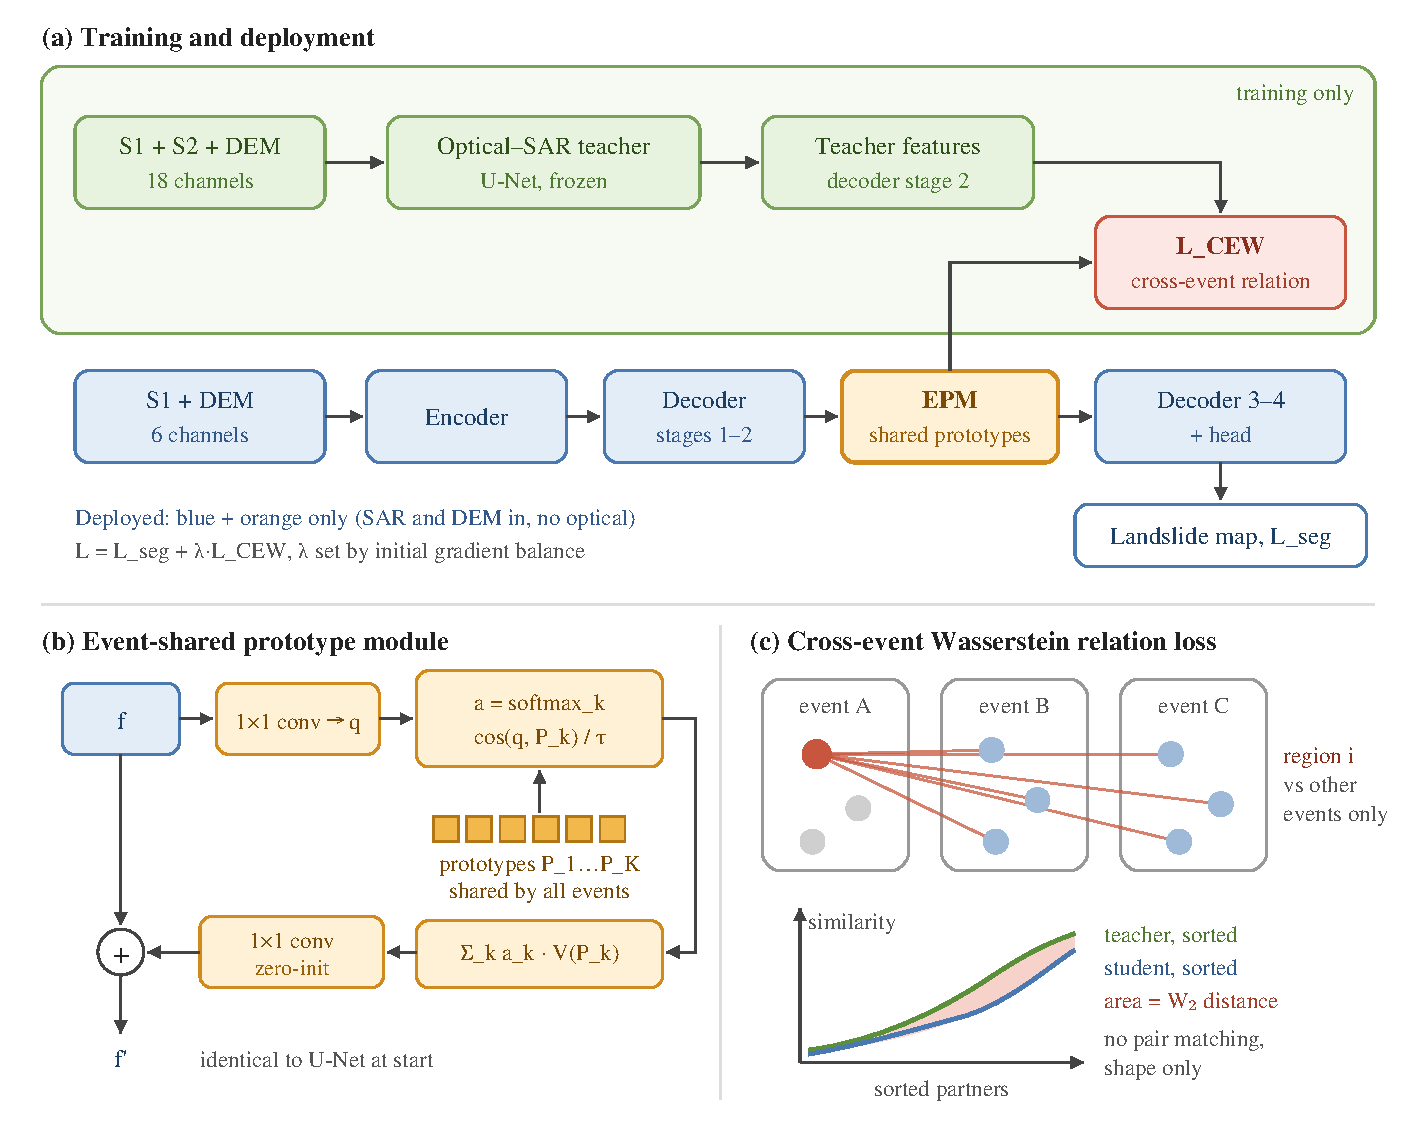
\includegraphics[width=0.92\textwidth]{figures_dlr/method.pdf}
\caption{(a) Training and deployment. The optical--SAR teacher (green) is used only during training. (b) Event-shared prototype module. (c) Cross-event Wasserstein relation loss: each region is compared only with regions of other events; teacher and student similarities are sorted separately and compared as distributions.}
\label{fig:method}
\end{figure*}

\subsection{Event-Shared Prototypes}
After the second decoder stage, the student feature $f\in\mathbb{R}^{C\times H\times W}$ is compared with $K$ learnable prototypes $\{P_k\}$ shared by all events:
\begin{equation}
a_k(p)=\mathrm{softmax}_k\!\left(\cos\bigl(W_q f(p),P_k\bigr)/\tau\right),
\label{eq:assign}
\end{equation}
\begin{equation}
f'(p)=f(p)+W_o\sum_k a_k(p)\,W_vP_k ,
\label{eq:refine}
\end{equation}
where $W_q$, $W_v$, and $W_o$ are $1\times1$ projections, $\tau=0.1$, and $K=16$. $W_o$ is zero-initialized, so training starts from the plain U-Net. The prototypes are the only parameters that every pixel of every event reads, and they remain in the deployed network.

\subsection{Cross-Event Wasserstein Relation Distillation}
Both feature maps at this stage are average-pooled over valid pixels into $4\times4$ region tokens per patch and normalized to unit length, giving $t_i$ (teacher) and $s_i$ (student, from $f'$). For region $i$ from event $e_i$, let $\mathcal{N}_i=\{j: e_j\neq e_i\}$ be the regions of other events in the mini-batch. The teacher and student similarity sets are
\begin{equation}
\mathcal{T}_i=\{t_i^\top t_j\}_{j\in\mathcal{N}_i},\qquad \mathcal{S}_i=\{s_i^\top s_j\}_{j\in\mathcal{N}_i},
\end{equation}
each shifted by its minimum over cross-event pairs. Sorting each set separately gives $\tilde{\mathcal{T}}_i$ and $\tilde{\mathcal{S}}_i$, and the squared one-dimensional Wasserstein distance between the two empirical distributions is
\begin{equation}
L_{\mathrm{CEW}}=\frac{1}{N}\sum_i\frac{1}{|\mathcal{N}_i|}\sum_{r=1}^{|\mathcal{N}_i|}\bigl(\tilde{\mathcal{T}}_i[r]-\tilde{\mathcal{S}}_i[r]\bigr)^2 .
\label{eq:cew}
\end{equation}
Sorting removes pair correspondence: the student decides which regions of other events are close or distant, while the teacher prescribes how the cross-event similarities are distributed. Same-event pairs never enter the loss, so acquisition conditions shared within an event cannot satisfy it.

\subsection{Learning Objective}
The student minimizes
\begin{equation}
L=L_{\mathrm{BCE}}+L_{\mathrm{Dice}}+\lambda L_{\mathrm{CEW}},
\label{eq:loss}
\end{equation}
with binary cross-entropy and foreground soft Dice on valid pixels. $\lambda$ is fixed before training from the gradient norms at initialization [TO FINALIZE: rule and value of the selected configuration].

\section{Experiments}
\subsection{Dataset and Settings}
We use the Sentinel-1/2 landslide reference data of~\cite{Orynbaikyzy2025} with its official split: 355 training and 88 validation patches from 23 events, and 120 test patches of $128\times128$ pixels at 10~m. The test set contains 44 patches from four independent events (Ind.) and 76 patches from four dependent events whose training patches are separated by a spatial block split (Dep.). Inputs follow the one-pre/one-post setting of~\cite{Orynbaikyzy2025}: $\gamma^0$ VV/VH in decibels, Copernicus DEM elevation, and slope; the teacher adds Sentinel-2 B2, B3, B4, B8, B11, and B12.

All networks use the U-Net of~\cite{Orynbaikyzy2025}, AdamW with a learning rate of $10^{-4}$ and weight decay of 0.01, batches of 16, random flips and rotations, and 200 epochs (constant rate for 100 epochs, then cosine decay). Validation IoU every 20 epochs selects the checkpoint; each model is tested once after selection, with threshold 0.5. All students share one initialization and the same frozen teacher (70.38\% test IoU). We report AP and pixel-pooled IoU and F1 over the test set, and IoU on Ind. and Dep.

\subsection{Main Comparison}
\begin{table}[!t]
\caption{Test results (\%) with SAR and terrain input at inference. KD methods share the student, initialization, and frozen optical--SAR teacher.}
\label{tab:main}
\centering\footnotesize
\setlength{\tabcolsep}{4pt}
\begin{tabular}{@{}lrrrrr@{}}
\toprule
Method & AP & IoU & F1 & IoU Ind. & IoU Dep. \\
\midrule
U-Net~\cite{Orynbaikyzy2025} & 72.91 & 52.20 & 68.59 & 63.24 & 46.03 \\
Vanilla KD~\cite{Hinton2015} & 70.89 & 53.45 & 69.66 & 68.52 & 44.97 \\
AT~\cite{Zagoruyko2017} & 76.63 & 53.12 & 69.39 & 61.22 & 48.63 \\
Multi-to-Uni~\cite{Sun2027} & 74.92 & 53.28 & 69.52 & 63.14 & 47.88 \\
ACAM-KD~\cite{Lan2025ACAM} & 74.54 & 54.59 & 70.63 & 66.09 & 48.45 \\
PKDOT~\cite{Aslam2024PKDOT} & 74.75 & 55.74 & 71.58 & 70.52 & 47.80 \\
DIS2~\cite{Kieu2026DIS2} & 75.85 & 55.97 & 71.77 & 69.71 & 48.06 \\
\textbf{Ours} & \textbf{\oursAP} & \textbf{\oursIoU} & \textbf{\oursFone} & \textbf{\oursInd} & \oursSpt \\
\midrule
Optical--SAR teacher & 85.09 & 70.38 & 82.62 & 81.90 & 64.88 \\
\bottomrule
\end{tabular}
\end{table}

Table~\ref{tab:main} compares distillation methods that transfer outputs (Vanilla KD), attention or features (AT, Multi-to-Uni, ACAM-KD, DIS2), and pairwise relations (PKDOT). [TO FINALIZE after the configuration is fixed: margin over each method; recall/precision $\oursR/\oursP$ versus U-Net $58.4/83.1$; discussion of Ind. versus Dep.]

\subsection{Why Pairwise Relations Transfer Poorly}
For every training and validation region we take the 30 regions of other events that the teacher finds least similar and measure the share that a frozen student also ranks among its own 30 least similar. Across 13 students trained with the same recipe, this agreement correlates negatively with test IoU ($r=-0.70$; Fig.~\ref{fig:overlap}). The best students agree with the teacher less than the U-Net does, whereas losses that enforce pair correspondence raise the agreement to 0.68--0.82 and test IoU falls to 52--53\%. Pairwise teacher relations therefore carry structure tied to the training events; the distribution of cross-event similarities is what transfers.

\begin{figure}[!t]
\centering
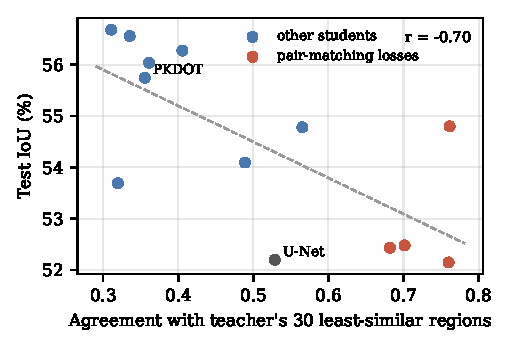
\includegraphics[width=\columnwidth]{figures_dlr/overlap.pdf}
\caption{Teacher--student agreement on the teacher's 30 least similar cross-event regions (validation patches) versus test IoU for students trained with the same recipe.}
\label{fig:overlap}
\end{figure}

\subsection{Ablation Study}
\begin{table}[!t]
\caption{Ablation (\%). All rows use the same U-Net, initialization, teacher, and recipe.}
\label{tab:ablation}
\centering\footnotesize
\begin{tabular}{@{}lrr@{}}
\toprule
Configuration & AP & IoU \\
\midrule
U-Net & 72.91 & 52.20 \\
+ prototypes (no optical) & 74.94 & 54.78 \\
+ $L_{\mathrm{CEW}}$ (no prototypes) & 76.41 & 55.57 \\
+ prototypes + $L_{\mathrm{CEW}}$ (Ours) & \oursAP & \oursIoU \\
\midrule
\multicolumn{3}{@{}l}{\emph{Relation target, with prototypes}} \\
Pairwise, rank-stratified partners & 72.55 & 52.43 \\
Pairwise, soft correspondence (KL) & 72.43 & 52.48 \\
Distribution, Wasserstein (Ours) & \oursAP & \oursIoU \\
\midrule
\multicolumn{3}{@{}l}{\emph{Relation source, PKDOT loss}} \\
Label-defined relations & 74.96 & 54.09 \\
Optical-teacher relations & 74.75 & 55.74 \\
Optical, cross-event pairs only & 77.24 & 56.27 \\
\bottomrule
\end{tabular}
\end{table}

Table~\ref{tab:ablation} isolates each component. [TO FINALIZE: text; add the all-event variant of $L_{\mathrm{CEW}}$ if run.]

\subsection{Deployment Cost}
The prototype module adds 0.10\,M parameters and 0.09\,G multiply--accumulate operations (MACs) to the 31.05\,M-parameter, 12.07\,GMAC U-Net per $128\times128$ patch. The teacher and $L_{\mathrm{CEW}}$ are used only in training, so inference uses SAR and terrain alone.

\section{Conclusion}
For event-grouped landslide inventories, an optical teacher transfers best to a SAR student through the distribution of its cross-event relations rather than through outputs, features, or pairwise relations. Matching this distribution with a closed-form Wasserstein loss and storing it in event-shared prototypes improves SAR-only landslide mapping on new events at negligible deployment cost. [TO FINALIZE: limitations, single-run results.]

\bibliographystyle{template/IEEEtran}
\bibliography{references_dlr}
\end{document}
